\documentclass[a4paper,10pt]{article}
\usepackage[utf8]{inputenc}
\usepackage{gensymb}
\usepackage{amsmath}
\usepackage{graphicx}
\graphicspath{ {images/} }

\newcommand{\lbparagraph}[1]{\paragraph{#1}\mbox{}\\}
\newcommand{\lbsubsection}[1]{\subsection{#1}}
\newcommand{\lbhiddensubsection}[1]{\subsection*{#1}}

\newcommand{\eqsp}[1]{\quad\#\quad}

\title{Formelsammlung Physik BMT 14a}
\author{Lukas Dörig, Michelle Meyer, Yan Poblete}
\date{\today\\v1.0}

\begin{document}

\maketitle

\section*{Intro: Geometrie}

\lbhiddensubsection{Trigonometrie}

\lbparagraph{Generell}

\begin{tabular}{l|l}
    Variable & Beschreibung \\
    \hline
    H & Hypothenuse \\
    GK & Gegenkathete \\
    AK & Ankathete
\end{tabular}

\lbparagraph{Sinus}

\begin{equation}
    \sin{\alpha} = \frac{GK}{H}
    \eqsp{}
    H = \frac{GK}{\sin{\alpha}}
    \eqsp{}
    GK = \sin{\alpha} \times H
\end{equation}

\begin{equation}
    \frac{a}{\sin{\alpha}} = \frac{b}{\sin{\beta}} = \frac{c}{\sin{\gamma}}
\end{equation}

\lbparagraph{Cosinus}

\begin{equation}
    \cos{\alpha} = \frac{AK}{H}
    \eqsp{}
    H = \frac{AK}{\cos{\alpha}}
    \eqsp{}
    AK = \cos{\alpha} \times H
\end{equation}

\begin{gather}
    a^2 = b^2 + c^2 - 2bc \times \cos{\alpha}
    \eqsp{}
    b^2 = a^2 + c^2 - 2ac \times \cos{\beta}
    \\
    c^2 = a^2 + b^2 - 2ab \times \cos{\gamma}
\end{gather}

\lbparagraph{Tangens}

\begin{equation}
    \tan{\alpha} = \frac{GK}{AK}
    \eqsp{}
    AK = \frac{GK}{\tan{\alpha}}
    \eqsp{}
    GK = \tan{\alpha} \times AK
\end{equation}

\lbparagraph{Wechsel- und Stufenwinkel}

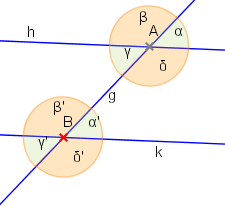
\includegraphics[height=103px,keepaspectratio]{stufen-wechselwinkel}

Wenn h $\parallel$ k. $\alpha$ und $\alpha$' sind Stufenwinkel, $\gamma$ und $\gamma$' sind Wechselwinkel.

%

\section{Kräftegelichgewicht, statisches Gleichgewicht}

\lbsubsection{Koordinaten}

\begin{tabular}{l l}
    Polarform & $(Betrag[F]|Winkel[\alpha])$ \\
    Karthesische Form & $(F_x|F_y)$
\end{tabular}

\lbparagraph{Polar zu Karthesisch}

\begin{equation}
    F_x = F \times \cos{\alpha}
    \eqsp{}
    F_y = F \times \sin{\alpha}
\end{equation}

\lbparagraph{Karthesisch zu Polar}

\begin{equation}
    F = \sqrt{F_x^2 + F_y^2}
    \eqsp{}
    \alpha = \arctan{\frac{F_y}{F_x}} + Sektor
\end{equation}

Für den Sektor muss jeweils addiert werden:

\begin{tabular}{l|l|l|r}
    Sektor & X Positiv? & Y Positiv? & Wert \\
    \hline
    1. & Ja & Ja & $0\degree$ \\
    2. & Nein & Ja & $90\degree$ \\
    3. & Nein & Nein & $180\degree$ \\
    4. & Ja & Nein & $270\degree$
\end{tabular}

\lbparagraph{Vektoren zusammenrechnen (Karthesisch)}

\begin{tabular}{l|l|l}		
  $F_1$ & $F_1x$ & $F_1y$ \\			
  $F_2$ & $F_2x$ & $F_2y$ \\			
  $F_3$ & $F_3x$ & $F_3y$ \\
  \hline
  $F_{res}$ & $F_{res}x$ & $F_{res}y$ \\
\end{tabular}

\lbsubsection{Kräfte}

\begin{tabular}{l|l}
    I & Alle Kräfte heben sich auf \\
    II & Alle Drehmomente heben sich auf
\end{tabular}

\lbparagraph{Im Allgemeinen}

\begin{equation}
    F = m \times a
    \eqsp{}
    [N] = [kg] \times [\frac{m}{s^2}] = [\frac{kg \times m}{s^2}]
\end{equation}

\lbparagraph{Schwerkraft}

\begin{equation}
    g = g_{Erde} = 9.81\frac{m}{s^2}
    \eqsp{}
    F_G = m \times g
\end{equation}

\lbparagraph{Hangabtriebskraft}

\begin{equation}
    F_H = F_G \times{\sin{\alpha}}
\end{equation}

\lbparagraph{Normalkraft}

\begin{equation}
    F_N = F_G \times \cos{\alpha}
\end{equation}

\lbparagraph{Reibungkraft}

\begin{equation}
    \mu = [Zahl, 0 - 1]
    \eqsp{}
    F_R = \mu \times F_N
\end{equation}

\lbparagraph{Federkraft}

\begin{equation}
    F_D = k \times x
    \eqsp{}
    F_D = D \times \Delta{s}
    \eqsp{}
    [N] = [\frac{N}{cm}] \times [cm]
\end{equation}

\lbparagraph{Fadenspannung}

\begin{gather}
    T = F_G + F \text{ (Bei hängender Masse)}
    \\
    F = T - F_R \text{ (Bei Masse auf Schiefer Ebene)}
\end{gather}

\lbsubsection{Drehmoment}

\lbparagraph{Generell}

\begin{tabular}{l|l|r}
    Variable & Beschreibung & Einheit \\
    \hline
    M & Drehmoment & [Nm] \\
    $F_{\perp}$ & Kraft, die senkrecht auf die Drehachse wirkt & [N]
\end{tabular}

\begin{equation}
    M = F_{\perp} \times l
\end{equation}

\lbparagraph{Statisch}


\begin{equation}
    F_{1\perp} \times l_1 = F_{2\perp} \times l_2
\end{equation}

\lbparagraph{In Bewegung}

\begin{equation}
    M_{Res} = M_{Uhrzeigersinn} - M_{Gegenuhrzeigersinn}
\end{equation}

\lbsubsection{Flaschenzug und Hebelgesetz}

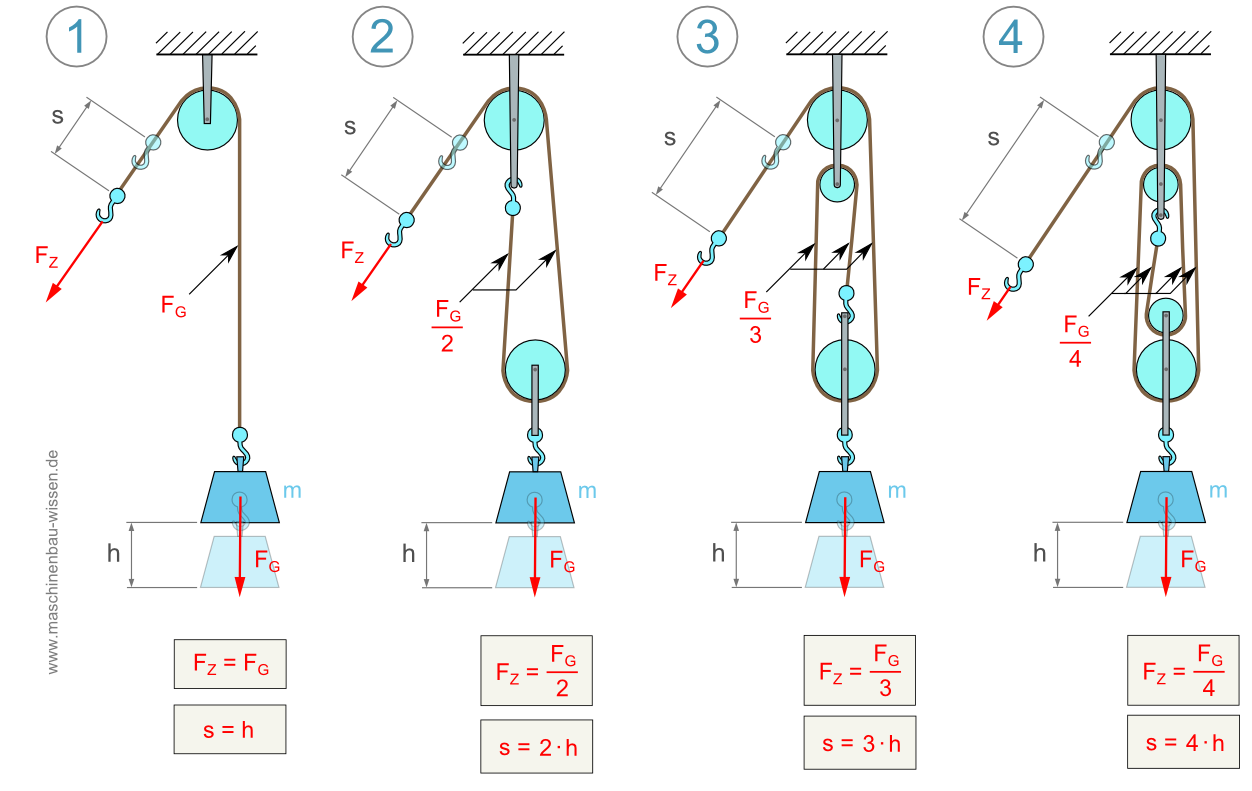
\includegraphics[width=\textwidth,height=\textheight,keepaspectratio]{flaschenzug-berechnen}

\lbsubsection{Hooksches Gesetz}

\lbparagraph{Parallel}

\[F = F_1 + F_2\]
\[k \times x = k_1 \times x + k_2 \times x\]
\[k = k_1 + k_2\]

\lbparagraph{Seriell}

\[F = F_1 = F_2 [???]\]
\[k = \frac{1}{\frac{1}{k_1} + \frac{1}{k_2}}\]
    
\section{Kinematik, Dynamik (Kraft)}

\lbsubsection{Kinematik}

\lbparagraph{Grundformeln}

\begin{tabular}{l|l|l}
    Variable & Formeln... & \\
    \hline
    $\overline{v}$ & $\frac{s}{t}$ & $\frac{v_0 + v}{2}$ \\
    \hline
    s & $\overline{v} \times t$ & $\frac{v_0 + v}{2} \times t$  \\
    \hline
    a & $\frac{v - v_0}{t}$ & \\
    \hline
    s & $s_0 + v_0 \times t + \frac{1}{2}a \times t^2$ & \\
    \hline
    $v^2$ & $v_0^2 + 2as$ & \\
    \hline
    v & $v_0 + at$ &
\end{tabular}

\lbparagraph{Varianten}

\begin{tabular}{l|l|l}
    Variable & Formeln... & \\
    \hline
    [???]
\end{tabular}

\lbsubsection{Drehung}

\lbparagraph{Variablendefinitionen}

\begin{tabular}{l|l|r|r}
    Variable & Beschreibung & Einheit & Weitere Einheiten \\
    \hline
    f & Drehfrequenz & Hz & $[\frac{1}{s}]$ \\
    T & Umlaufzeit & [s] & \\
    n & Anzahl Umdrehungen & [Zahl] &  \\
    b & Bogenlänge & [m] &  \\
    $\theta$ & Drehwinkel & [Radiant] & \\
    $\omega$ & Winkelgeschwindigkeit & $[\frac{1}{s}]$ & $[\frac{Radiant}{s}]$ \\
    $a_z$ & Zentripetalbeschleunigung & $[\frac{m}{s^2}]$ &  \\
    $F_z$ & Zentripetalkraf (=Zentrifugalkraft) & [N] &
\end{tabular}

\lbparagraph{Formeln}

\begin{tabular}{l|l|l|l}
    Variable & Formeln... & & \\
    \hline
    f & $\frac{1}{T}$ & $\frac{n}{\Delta{t}}$ &  \\
    \hline
    $\theta$ & $\frac{b}{r}$ & $\frac{2\pi \times \alpha}{360\degree}$ & $\omega \times t$ \\
    \hline
    $\alpha$ & $\frac{360\degree \times \theta}{2\pi}$ & & \\
    \hline
    $\omega$ & $\frac{\theta}{t}$ & $\frac{v}{r}$ & $2\pi \times f$ \\
    \hline
    v & $\frac{b}{t}$ & $\omega \times r$ & \\
    \hline
    b & $v \times t$ & $\omega \times rt$ & $\theta \times r$ \\
    \hline
    $a_z$ & $\frac{v^2}{r}$ & $\frac{(\omega \times r)^2}{r}$ & $\omega^2 \times r$ \\
    \hline
    $F_z$ & $a_z \times m$ & &
\end{tabular}

\lbparagraph{Weitere Umformungen}

[???]

\lbsubsection{Keplresche Gesetze}

\[F_G = \frac{G \times m_1 \times m_2}{r^2}\]

\lbsubsection{Bremsweg}

\[s_b = \frac{V_0^2}{2g\mu}\]

\section{Arbeit, Energie, Leistung}

\lbsubsection{Energieerhaltungssatz}

\lbparagraph{Variablendefinitionen}

\begin{tabular}{l|l|r|r}
    Variable & Beschreibung & Einheit & Weitere Einheiten \\
    \hline
    W & Arbeit & [J] & [Nm]  \\
    E & Energie (gespeicherte Arbeit) & [J] & [Nm] \\
    P & Leistung & [W] & $[\frac{J}{s}] = [\frac{Nm}{s}]$
\end{tabular}

\lbparagraph{Satz}

\begin{tabular}{l l l l}
    $E_{tot1}$ & $- E_{Verlust}$ & $+ E_{Zu}$ & $= E_{tot2}$  \\
    $E_{kin1} + E_{pot1} + E_{D1}$ & $- E_R$ & $+ E_{Zu}$ & $= E_{kin2} + E_{pot2} + E_{D2}$
\end{tabular}

\lbparagraph{Kinetische Energie}

\[E_{kin} = \frac{1}{2}mv^2\]

\lbparagraph{Potentielle Energie}

\[E_{pot} = mgh\]

\lbparagraph{Federenergie \ Deformationsenergie}

D: Federkonstante $[\frac{N}{cm}]$

\[E_D = \frac{1}{2}Ds^2\]

\lbparagraph{Reibungsenergie}

Horizontale: \[E_R = F_R \times s = \mu \times mg \times s\]

Schiefe Ebene: \[E_R = F_R \times s = \mu \times mg \times \cos{\alpha} \times s\]

\end{document}
